\documentclass{standalone}
\usepackage{pgfplots}
\begin{document}
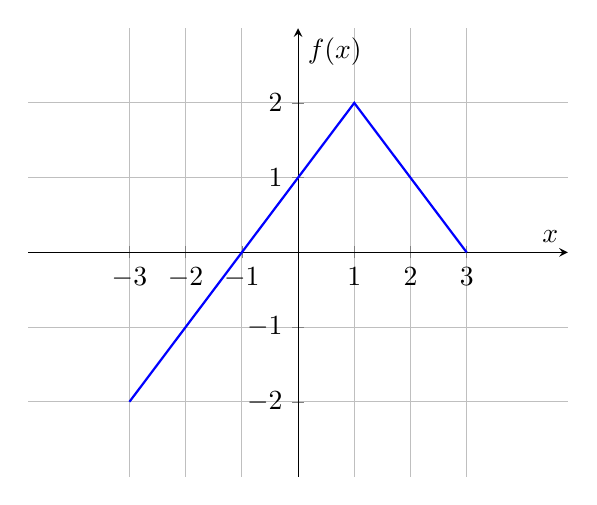
\begin{tikzpicture}
  \begin{axis}[
      axis lines=middle,
      xlabel={$x$},
      ylabel={$f(x)$},
      xmin=-4, xmax=4,
      ymin=-2.5, ymax=2.5,
      xtick={-3,-2,-1,0,1,2,3},
      ytick={-2,-1,0,1,2},
      grid=both,
      enlargelimits=true,
    ]
    % Plot the piecewise linear function
    \addplot[
      thick,
      blue,
      domain=-1:3
    ] coordinates {
       (-3,-2) (-1,0) (0,1) (1,2)  (3,0) 
    };
  \end{axis}
\end{tikzpicture}
\end{document}
